%----------------------------------------------------------------------------------------
%	PACKAGES AND THEMES
%----------------------------------------------------------------------------------------
\documentclass[aspectratio=169,xcolor=dvipsnames]{beamer}
\usetheme{SimplePlus}

\usepackage{hyperref}
\usepackage{graphicx} % Allows including images
\usepackage{booktabs} % Allows the use of \toprule, \midrule and \bottomrule in tables

%----------------------------------------------------------------------------------------
%	TITLE PAGE
%----------------------------------------------------------------------------------------

\title{PHD Tracking Result} % The short title appears at the bottom of every slide, the full title is only on the title page

\date{\today} % Date, can be changed to a custom date


%----------------------------------------------------------------------------------------
%	PRESENTATION SLIDES
%----------------------------------------------------------------------------------------

\begin{document}

\begin{frame}
    % Print the title page as the first slide
    \titlepage
\end{frame}

%------------------------------------------------
%------------------------------------------------

\begin{frame}{Issue One: Duplicated IDs}
    \begin{figure}
    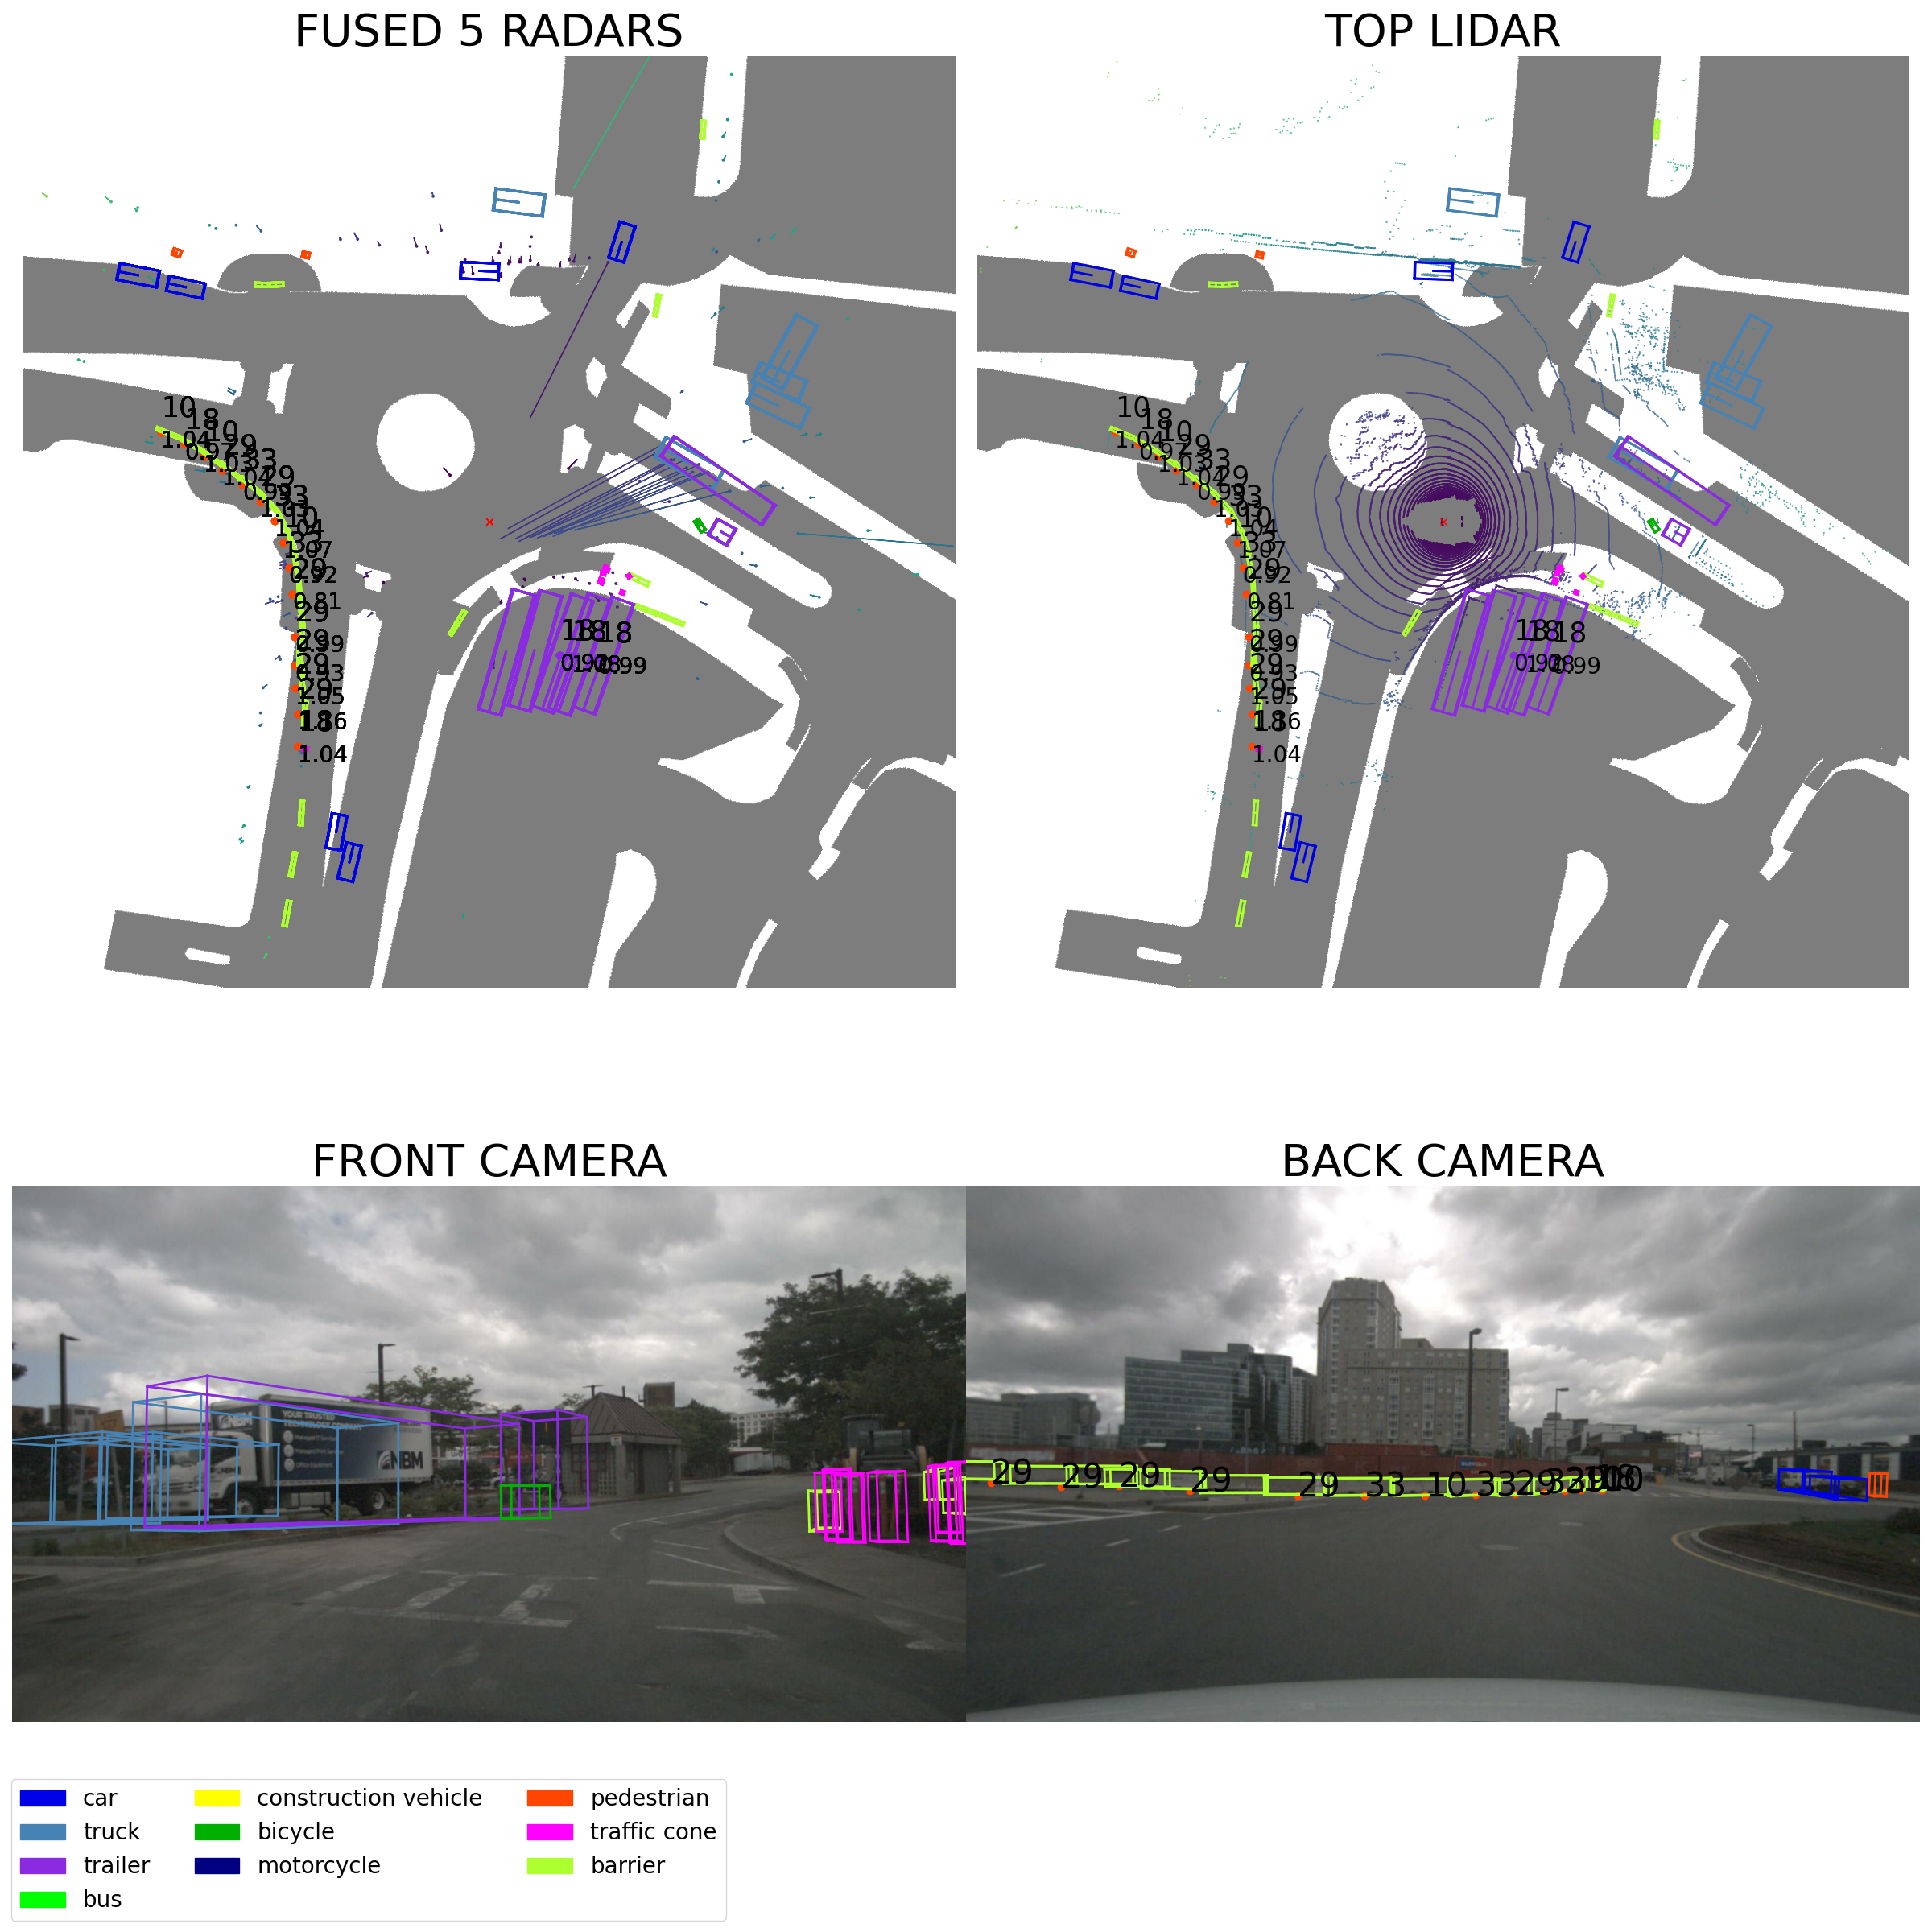
\includegraphics[width=0.5\linewidth]{issue1_duplicatedID.png}
    \end{figure}
\end{frame}

\begin{frame}{Issue Two: Frequent ID switches, LABEL}
    \begin{figure}
    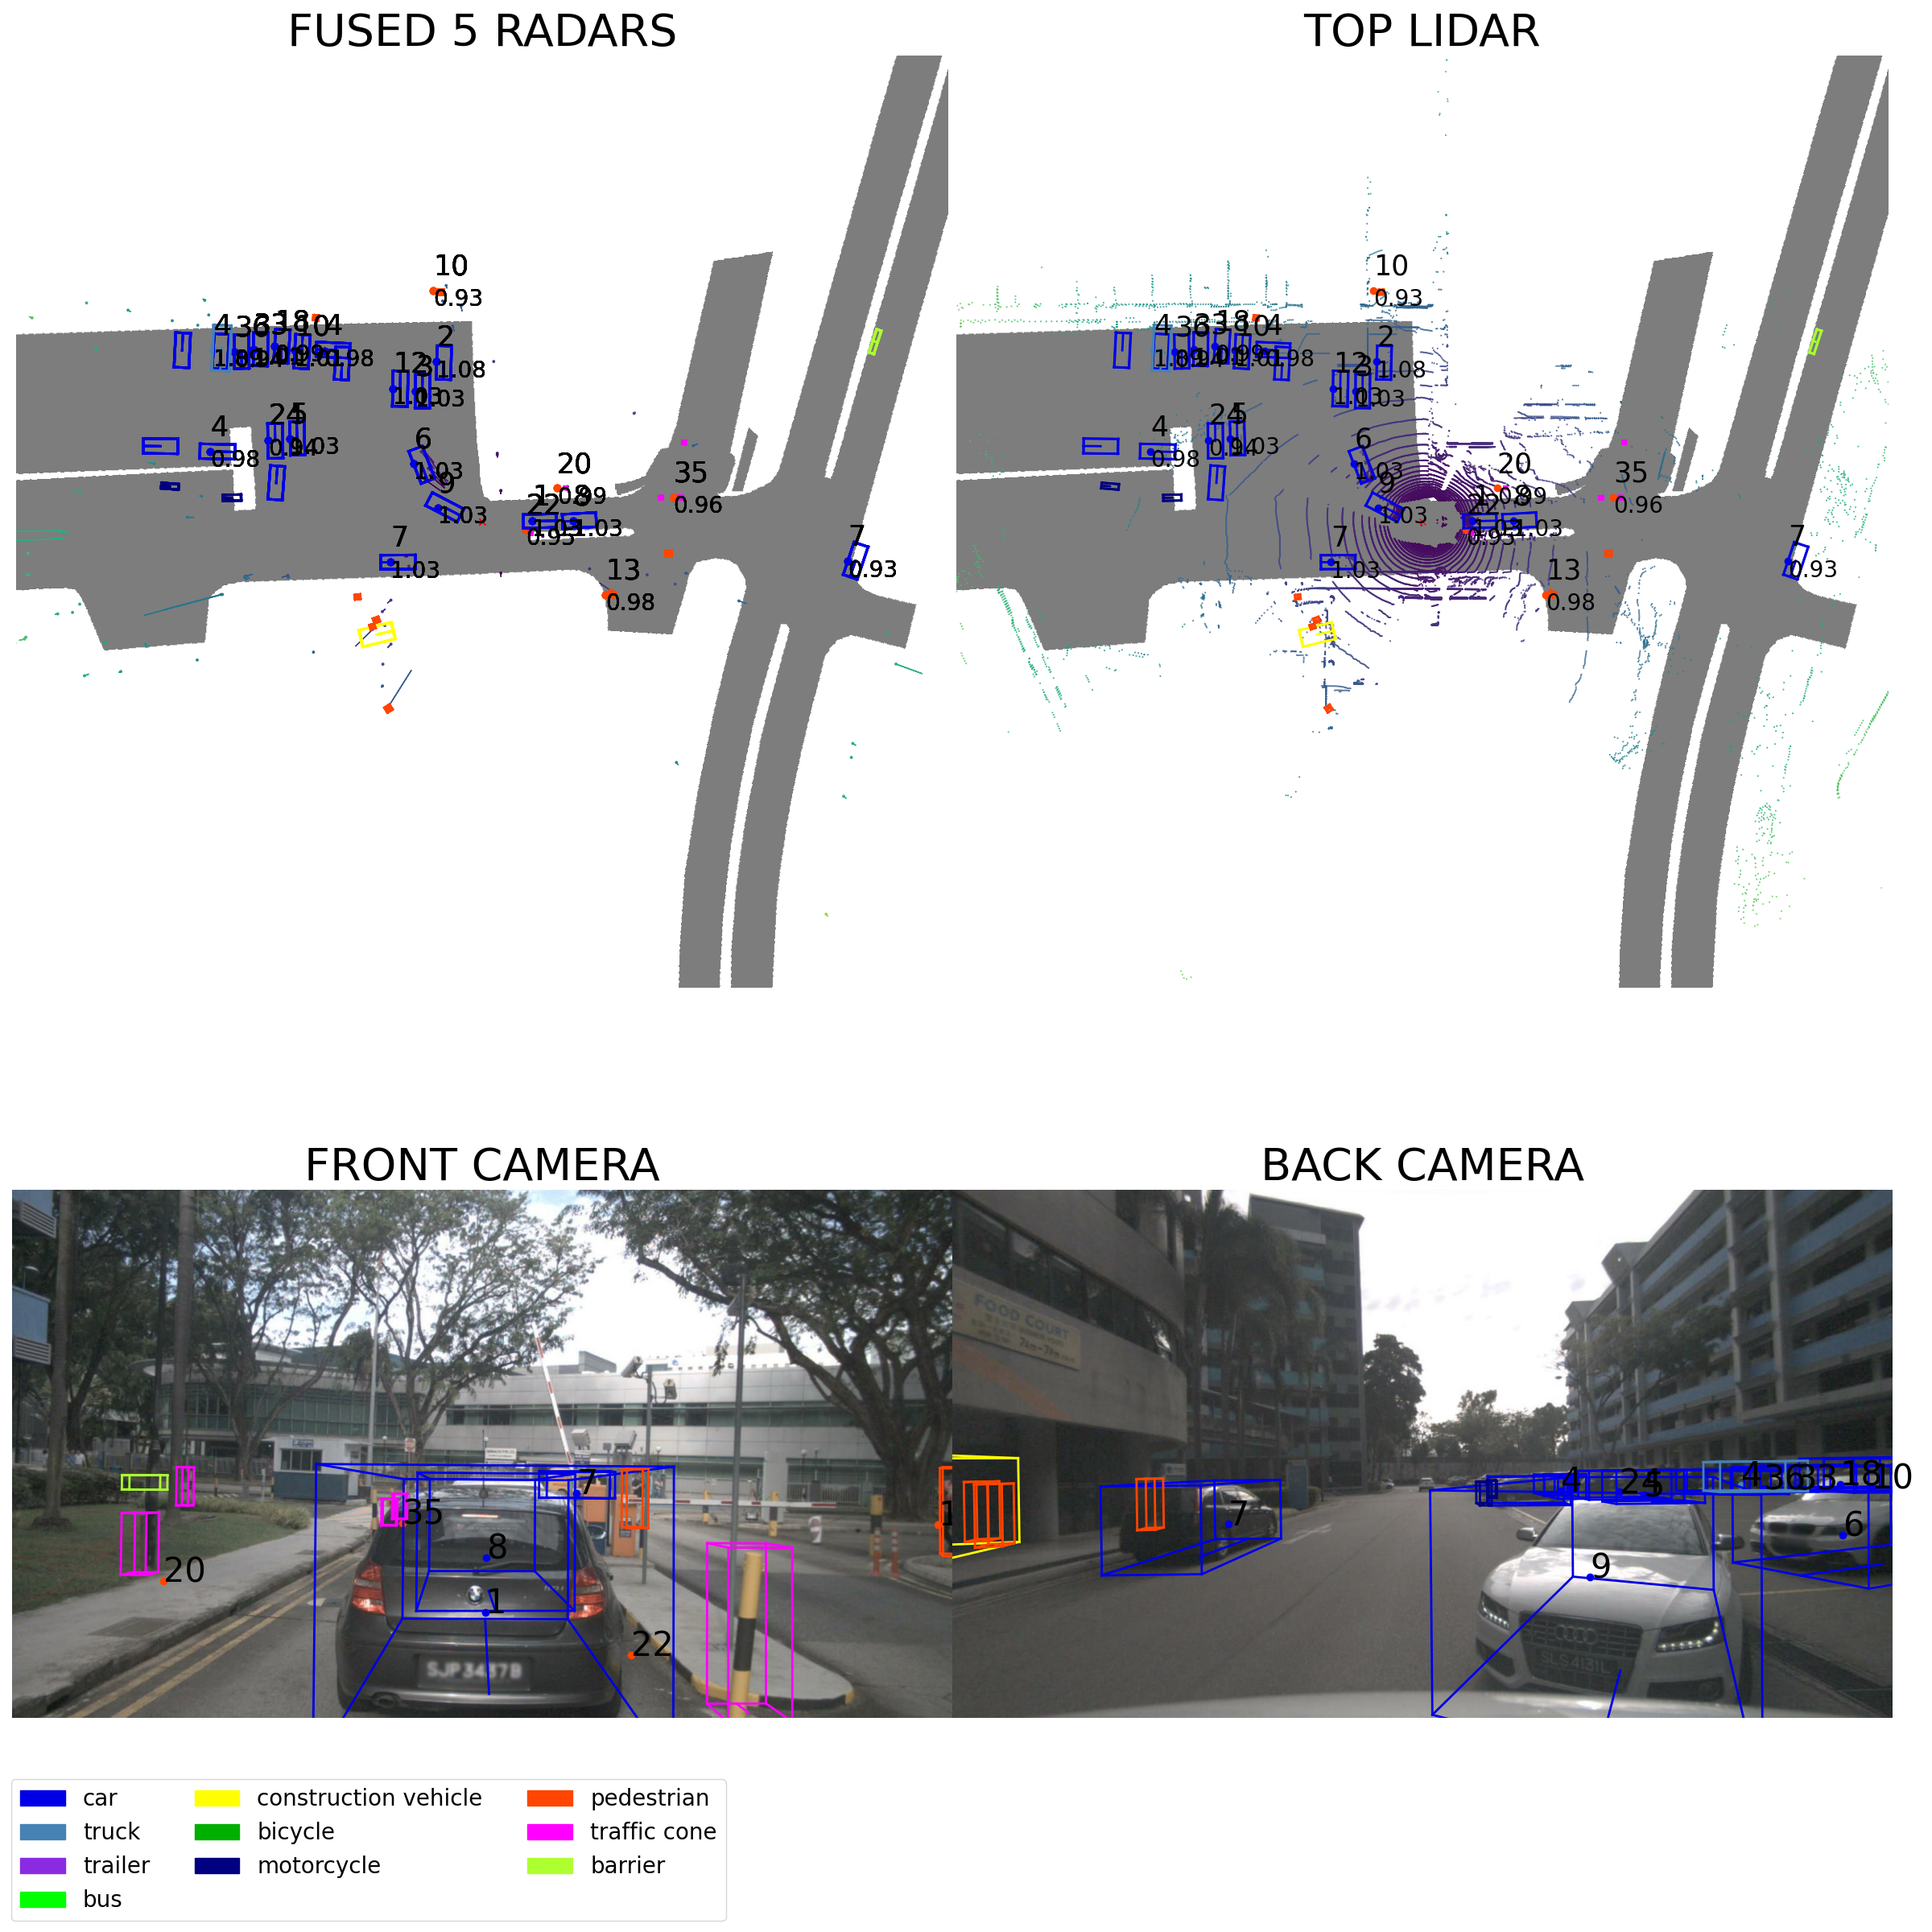
\includegraphics[width=0.5\linewidth]{label/1.png}
    \end{figure}
\end{frame}

\begin{frame}{Issue Two: Frequent ID switches, LABEL}
    \begin{figure}
    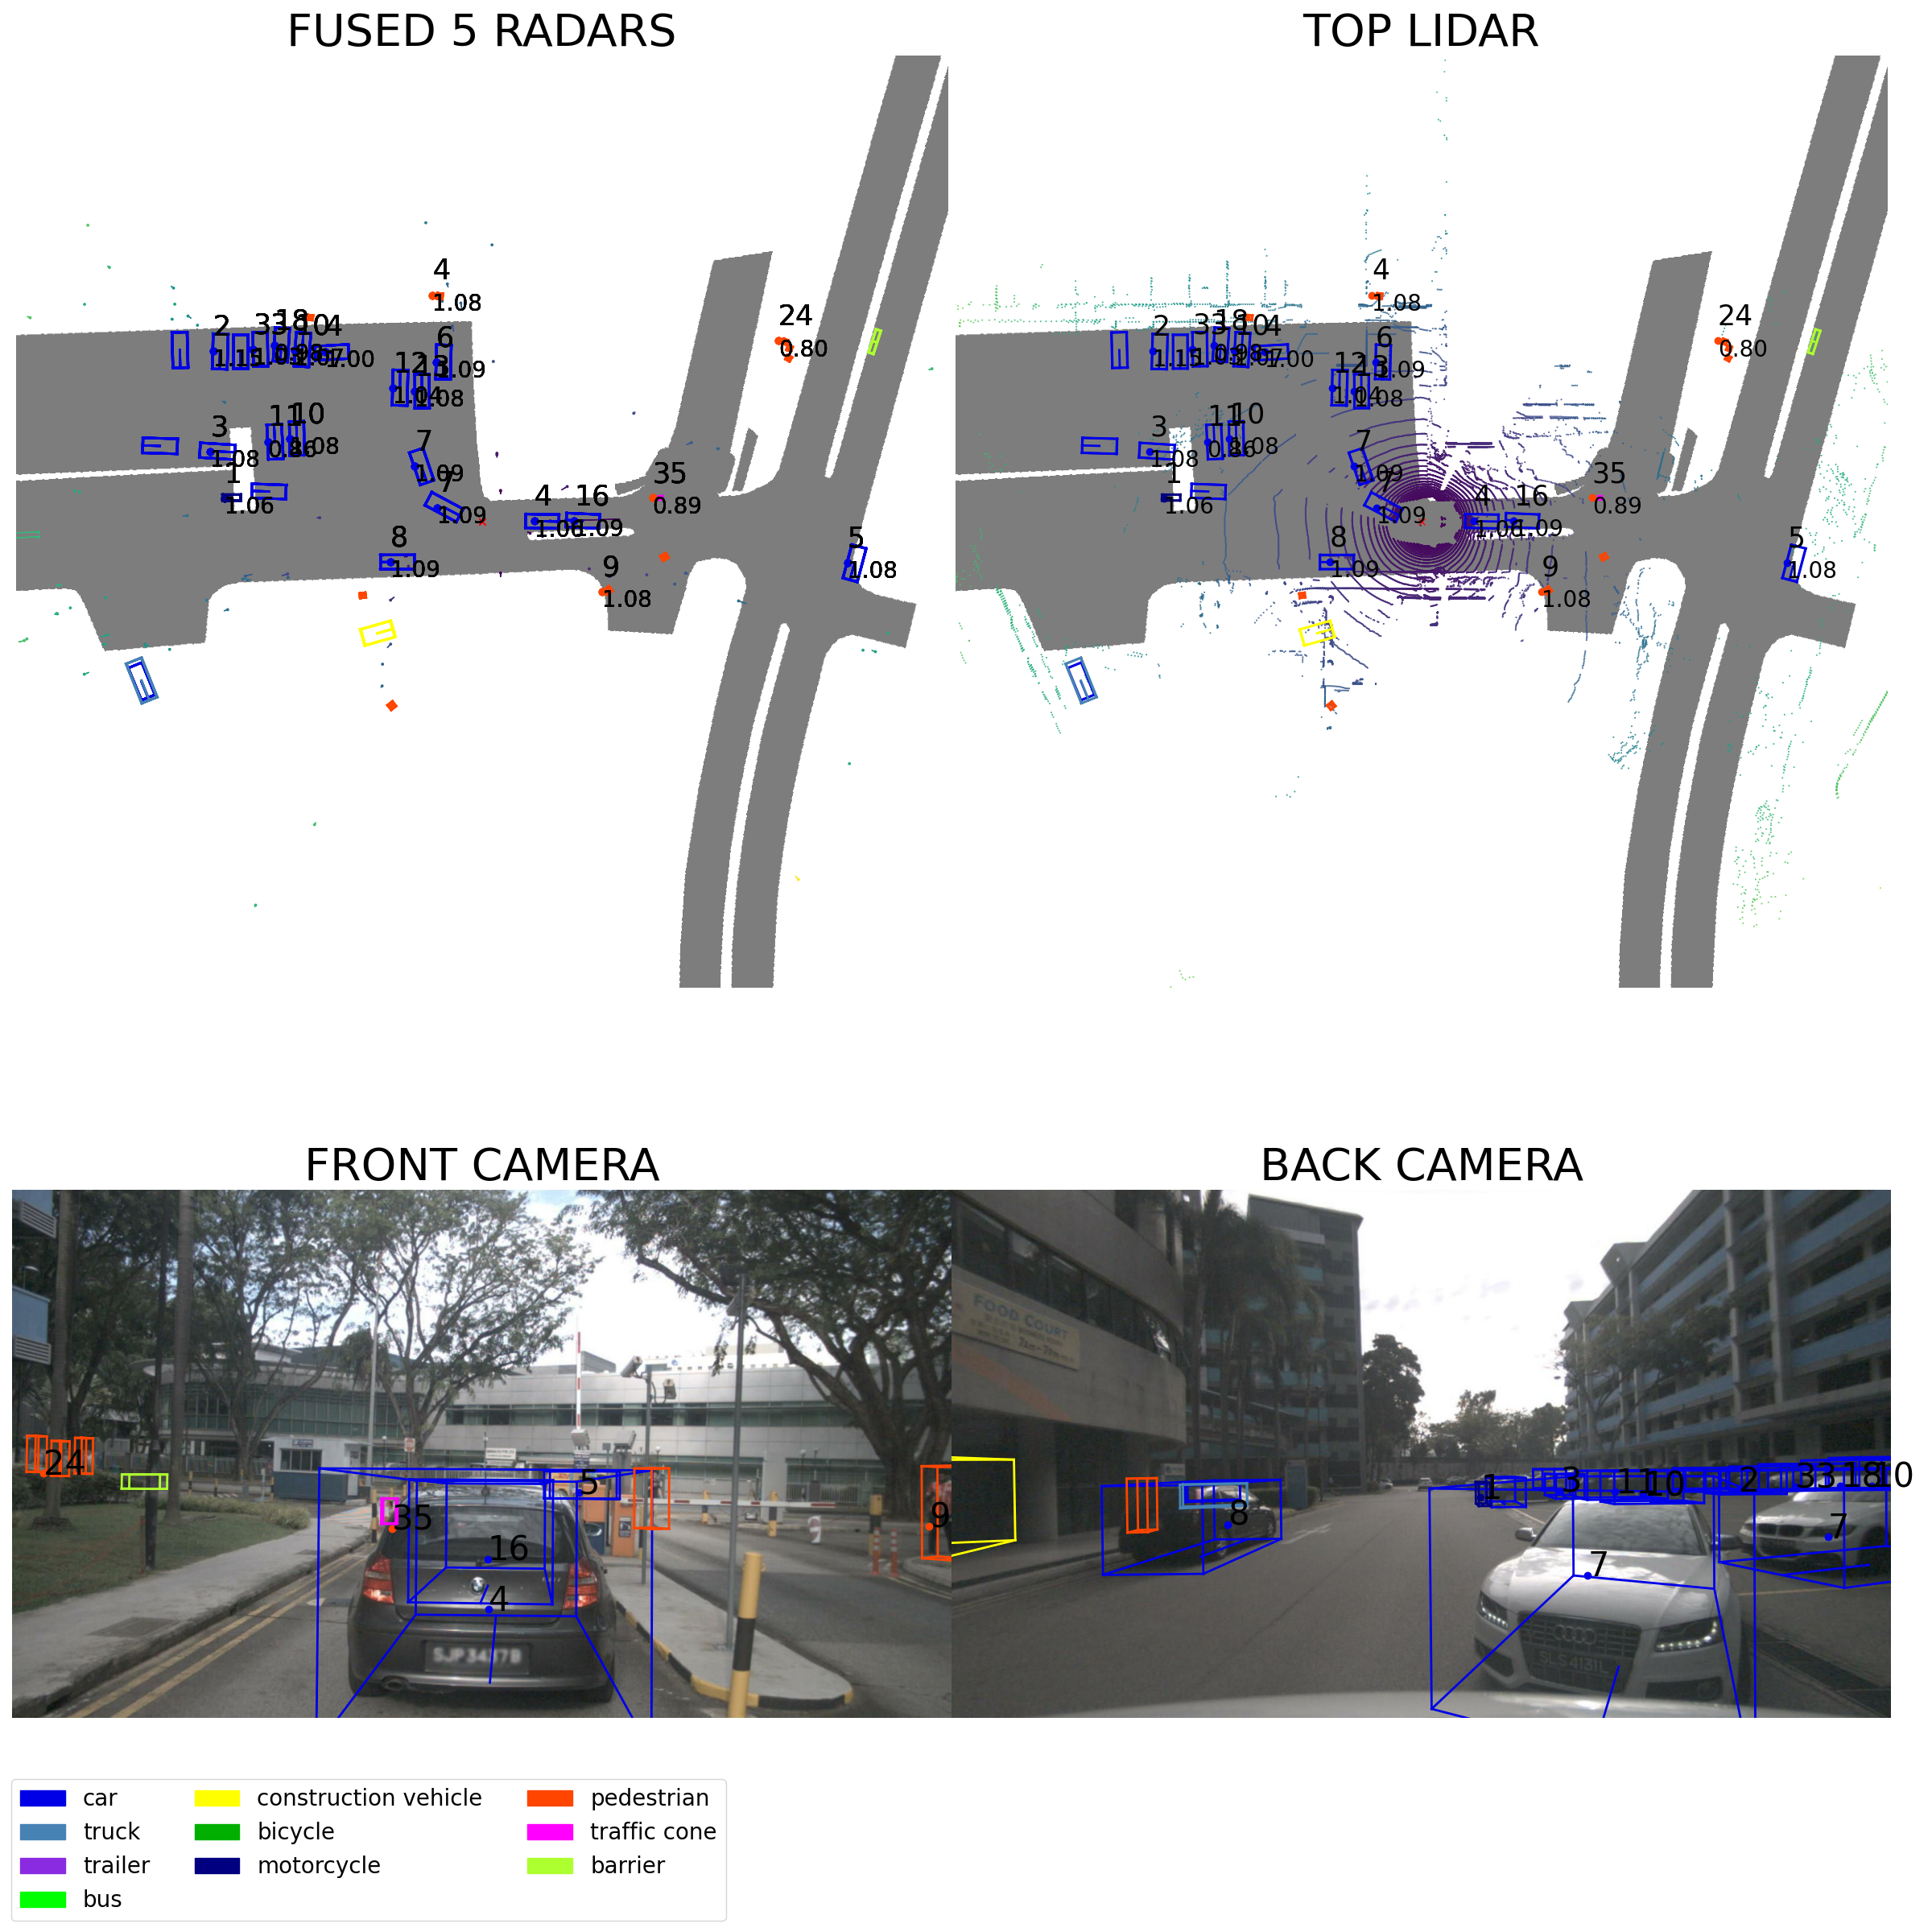
\includegraphics[width=0.5\linewidth]{label/2.png}
    \end{figure}
\end{frame}


\begin{frame}{Issue Two: Frequent ID switches, LABEL}
    \begin{figure}
    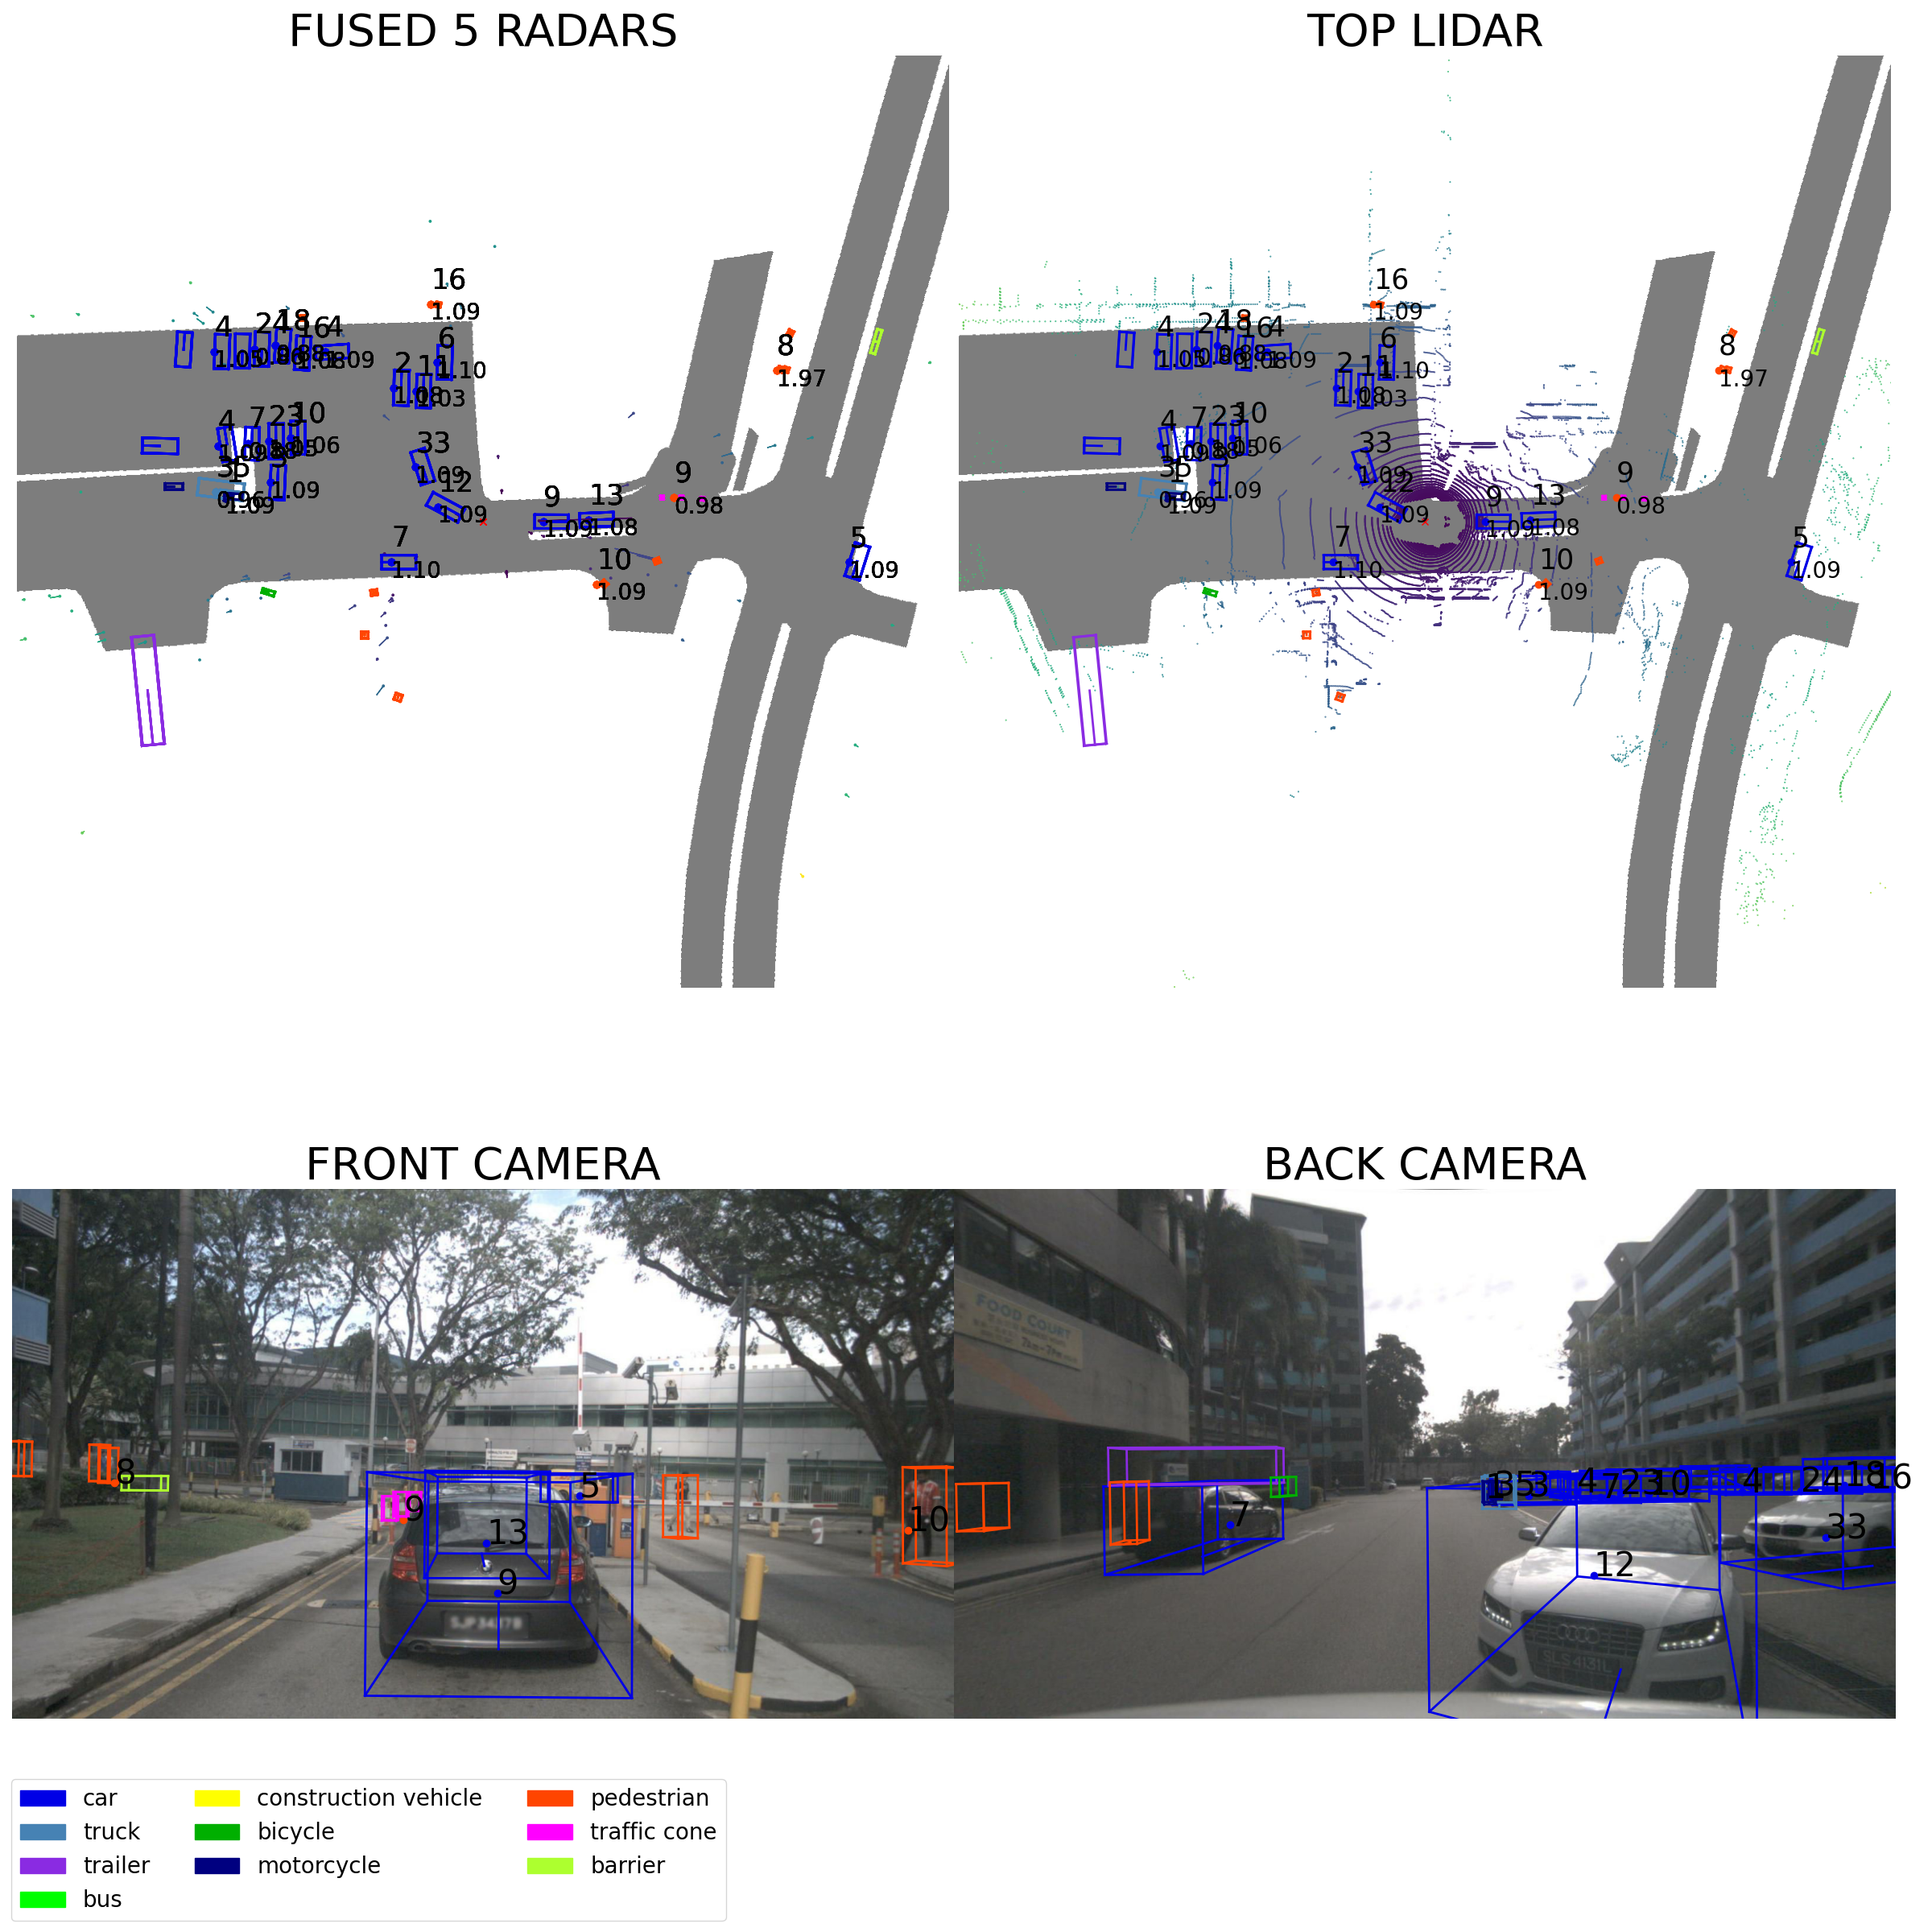
\includegraphics[width=0.5\linewidth]{label/4.png}
    \end{figure}
\end{frame}

\begin{frame}{Compare to: GNN Less Frequent ID switches}
    \begin{figure}
    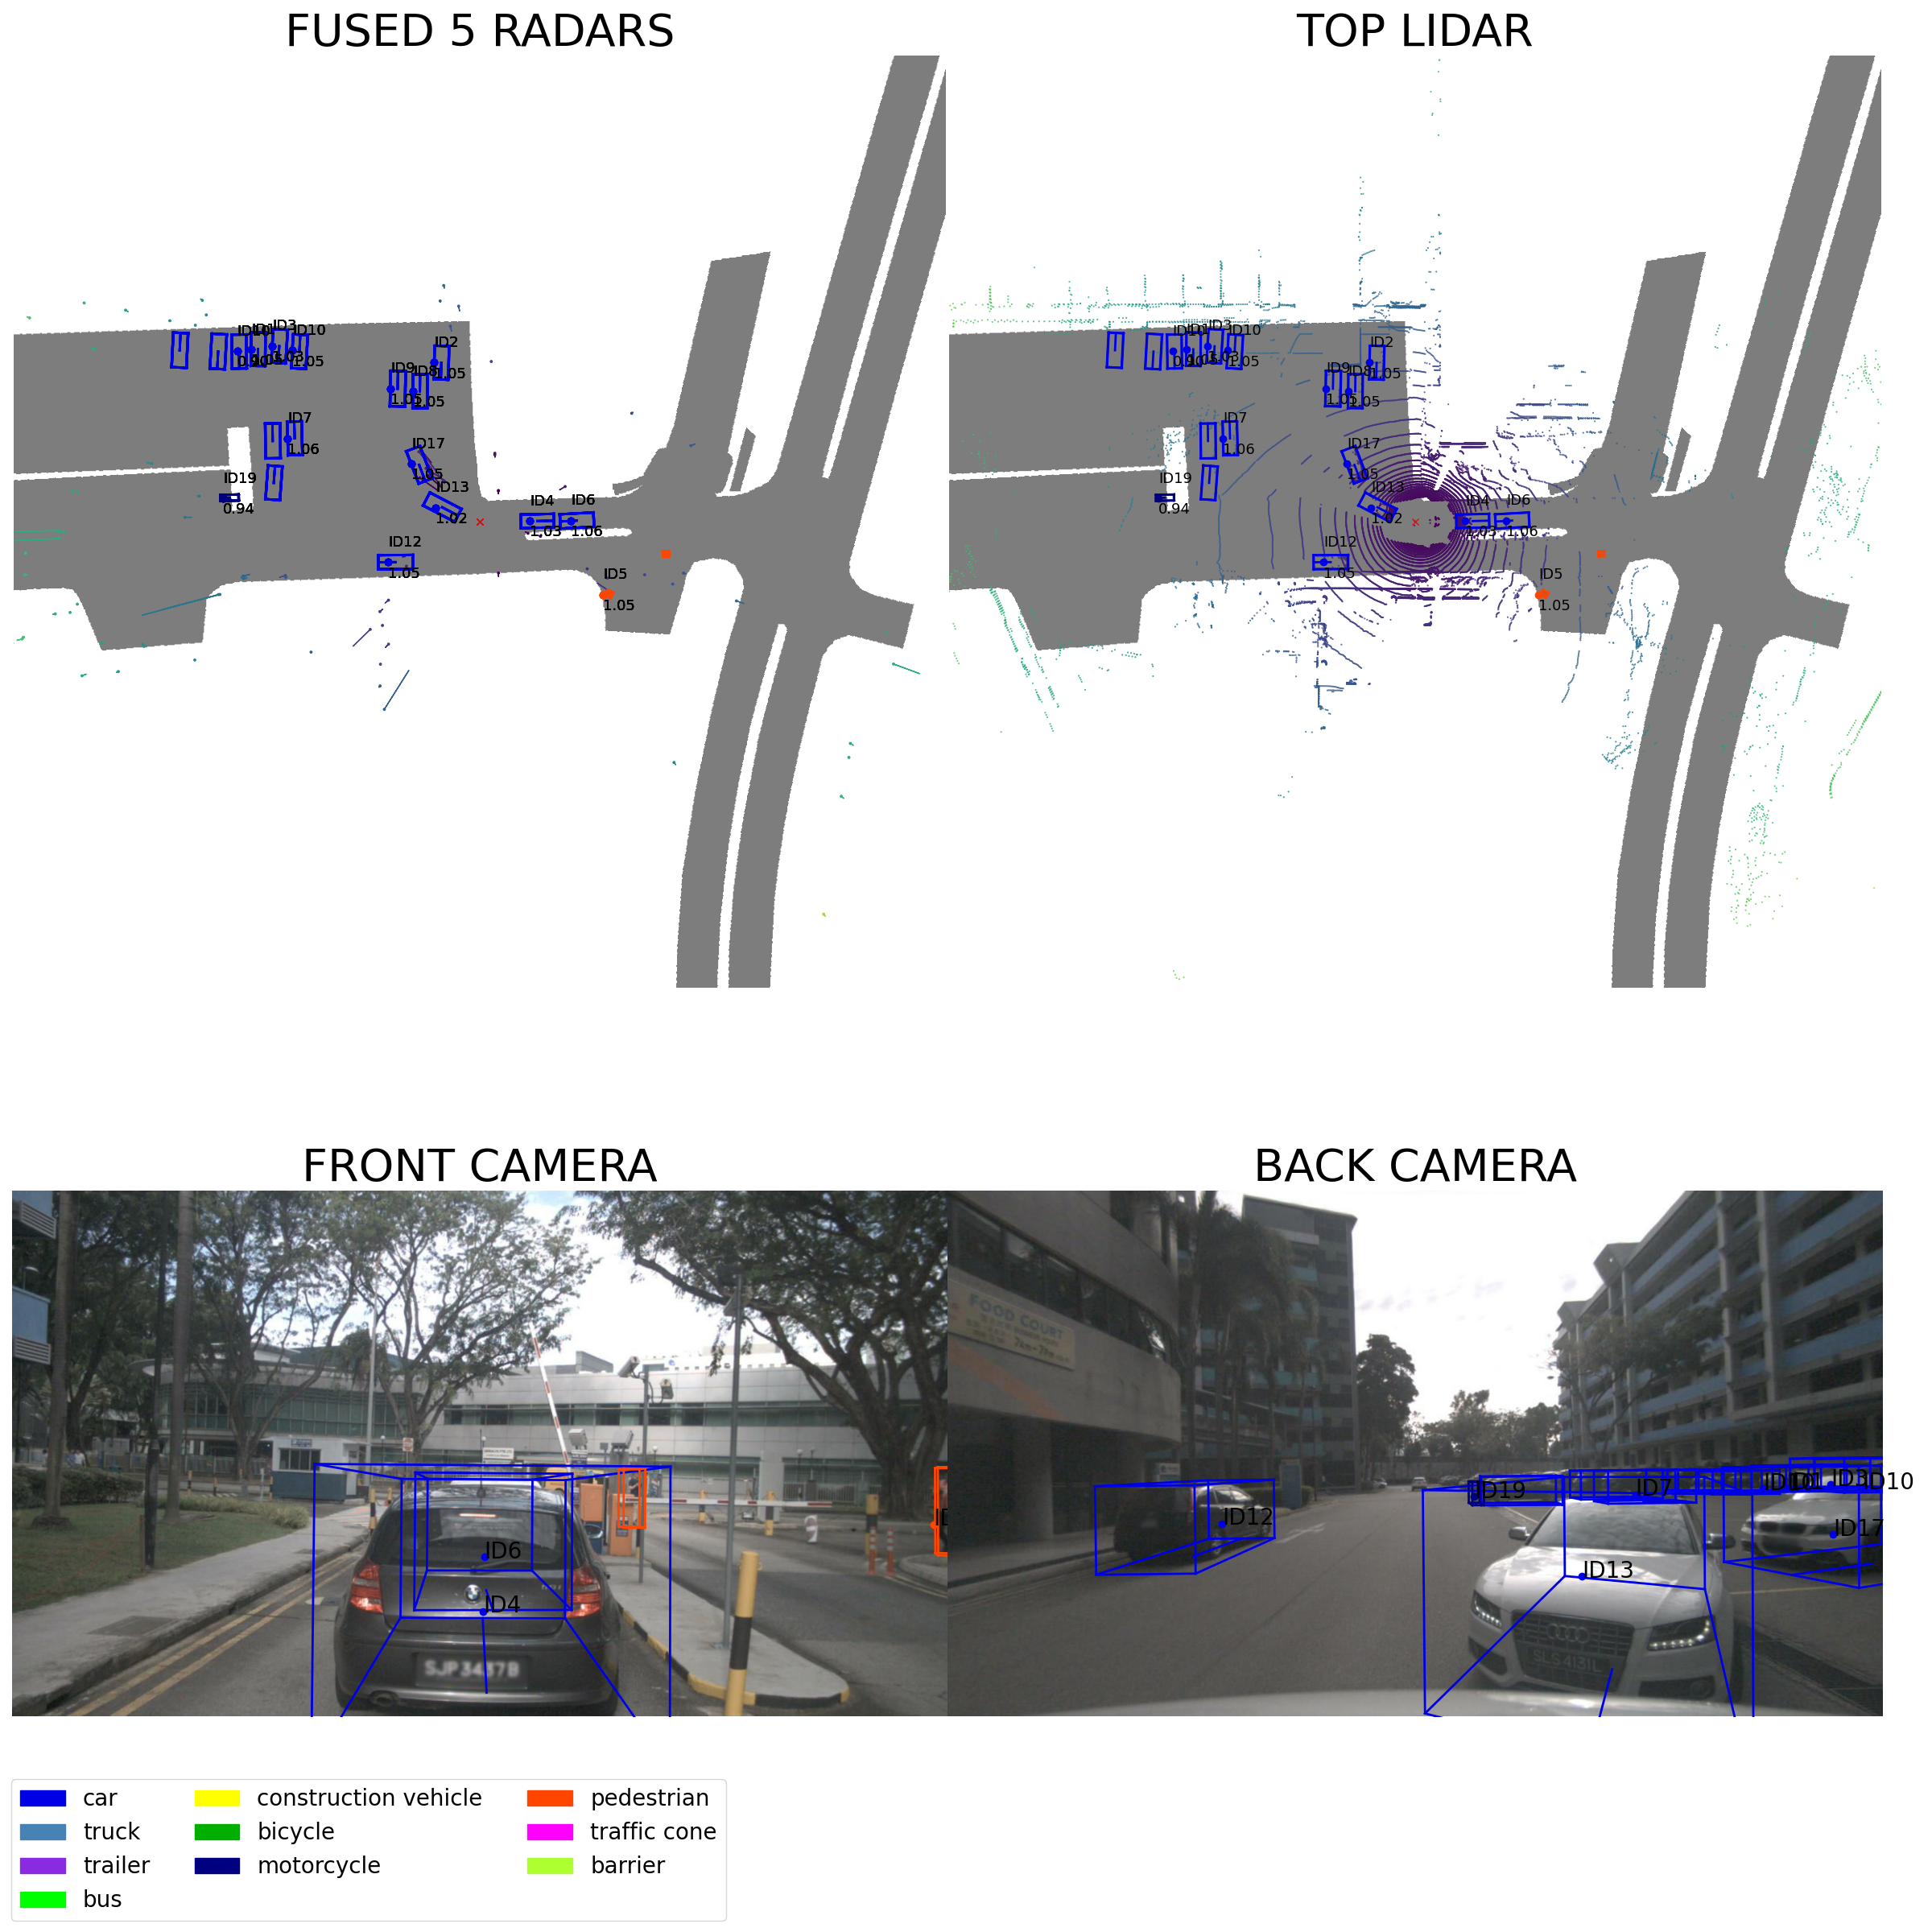
\includegraphics[width=0.5\linewidth]{GNN/1.png}
    \end{figure}
\end{frame}

\begin{frame}{Compare to: GNN Less Frequent ID switches}
    \begin{figure}
    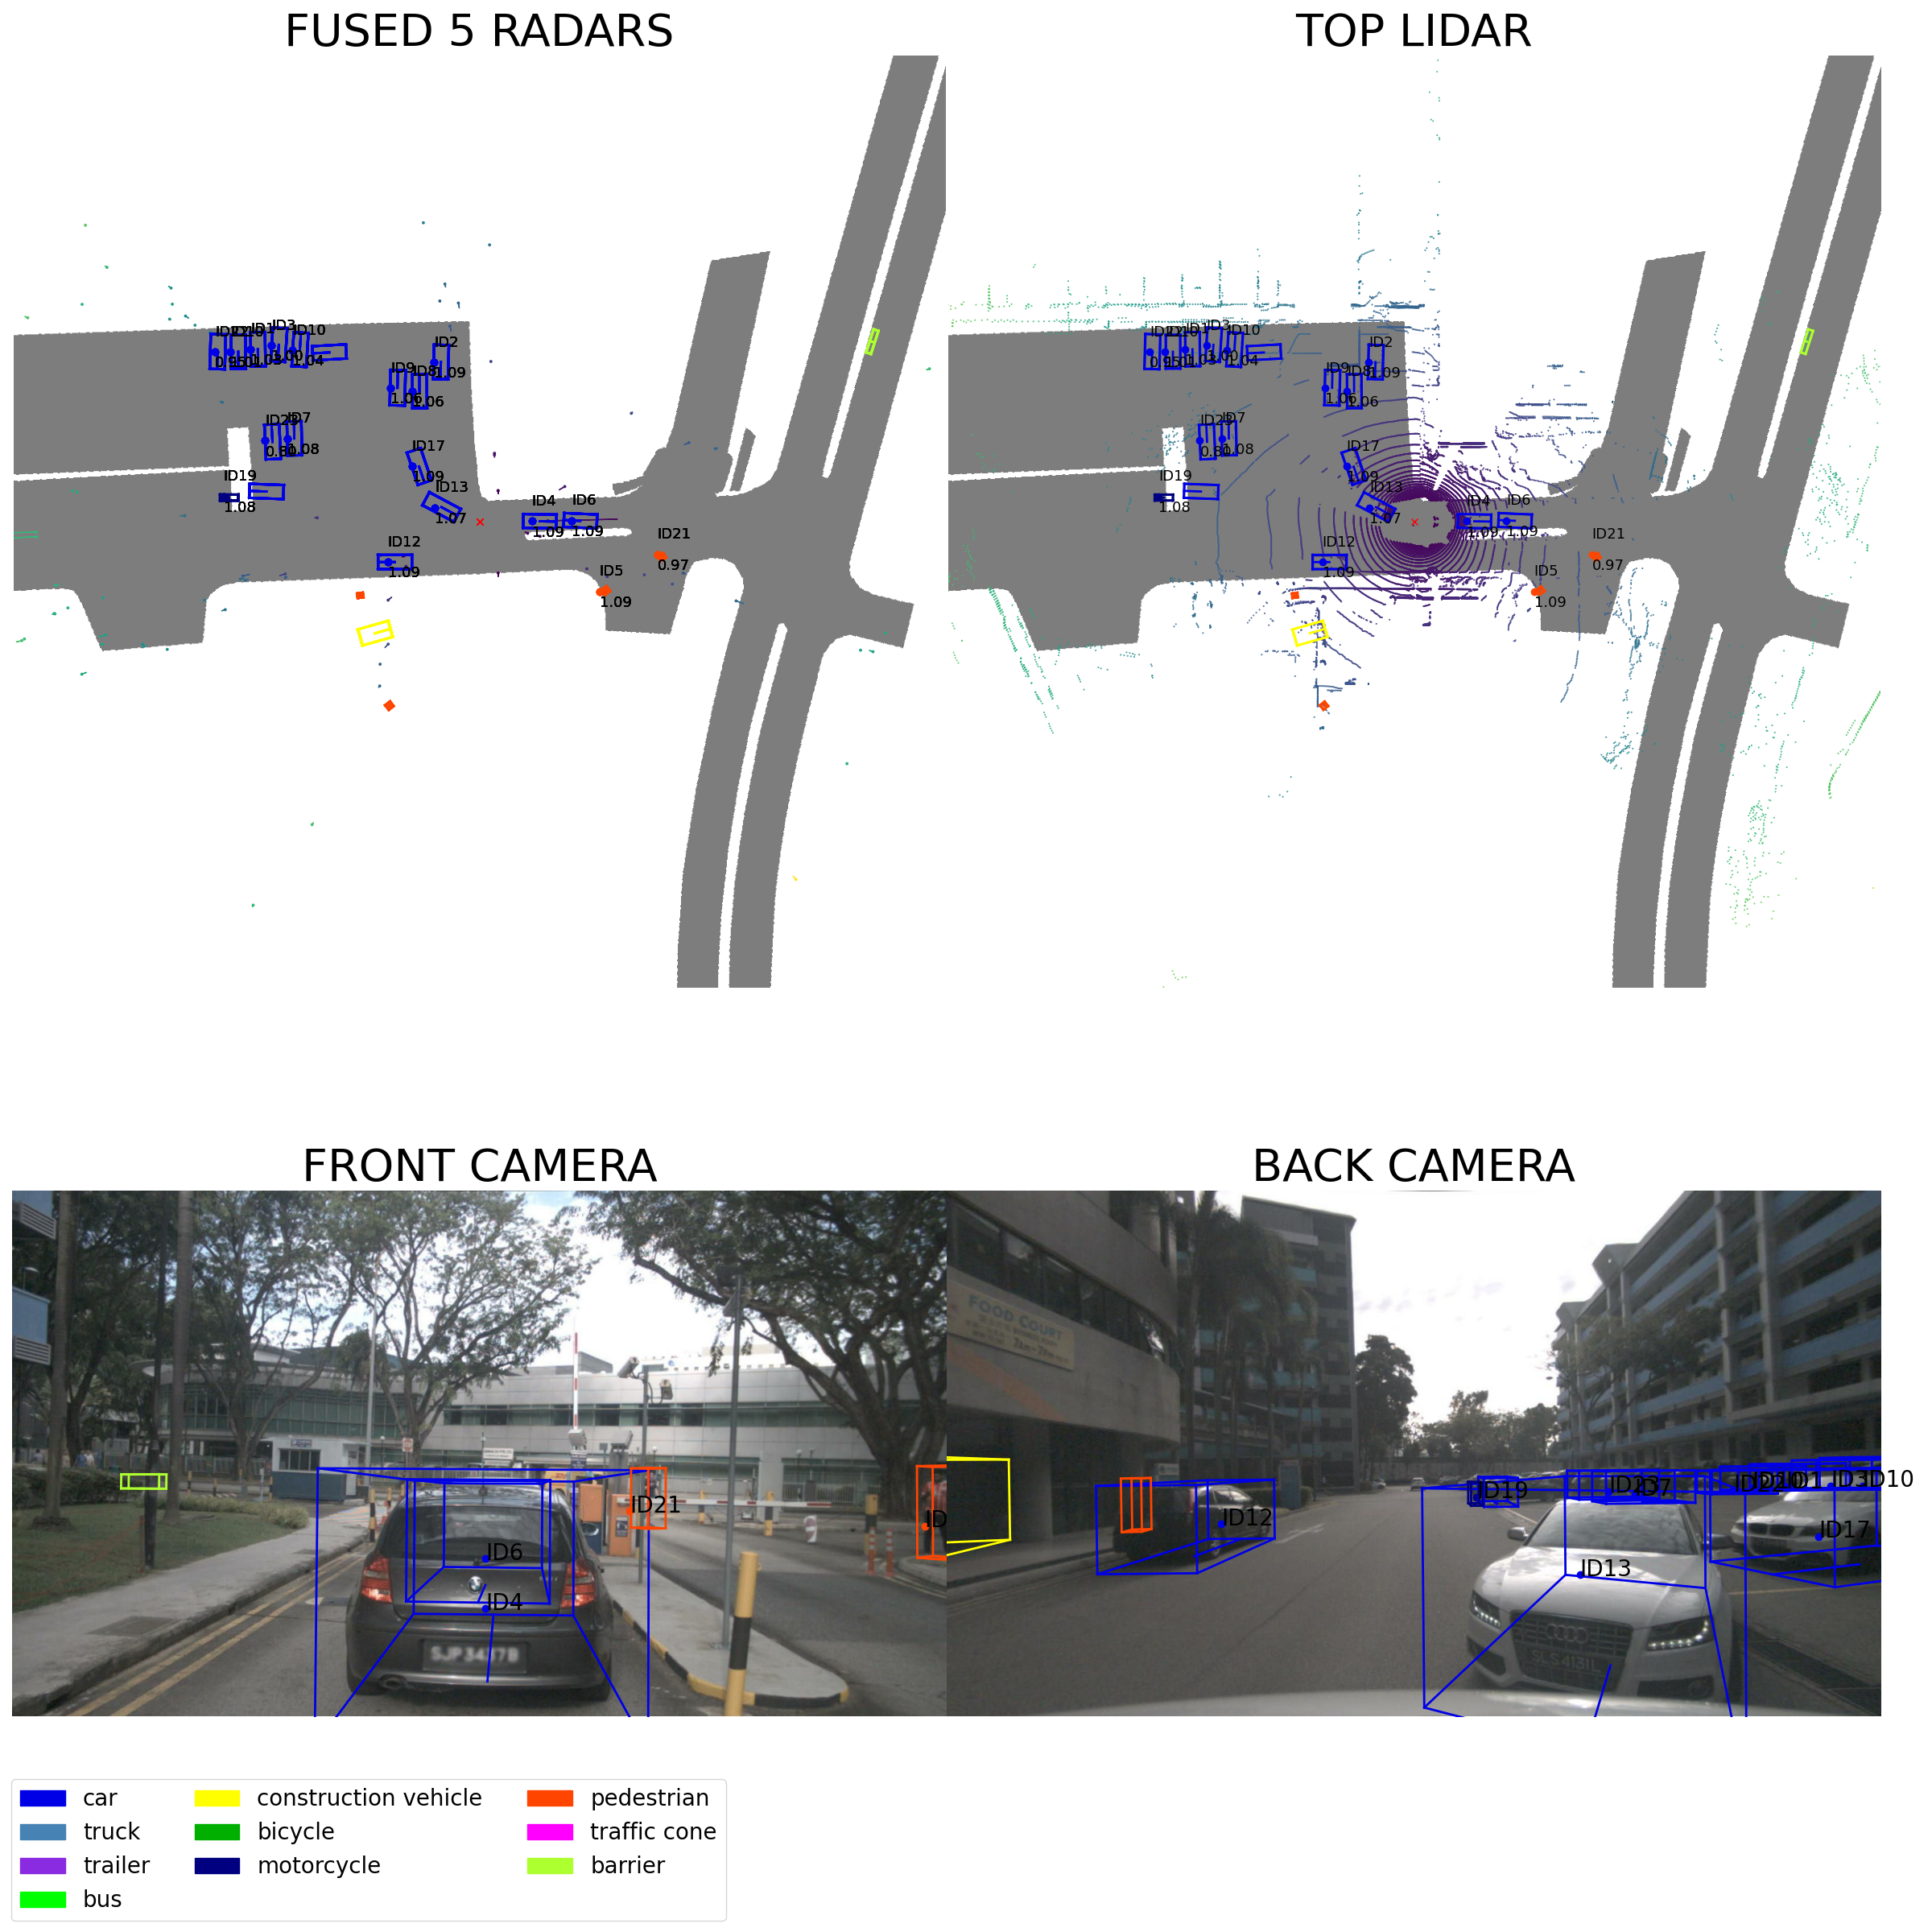
\includegraphics[width=0.5\linewidth]{GNN/2.png}
    \end{figure}
\end{frame}


\begin{frame}{Compare to: GNN Less Frequent ID switches}
    \begin{figure}
    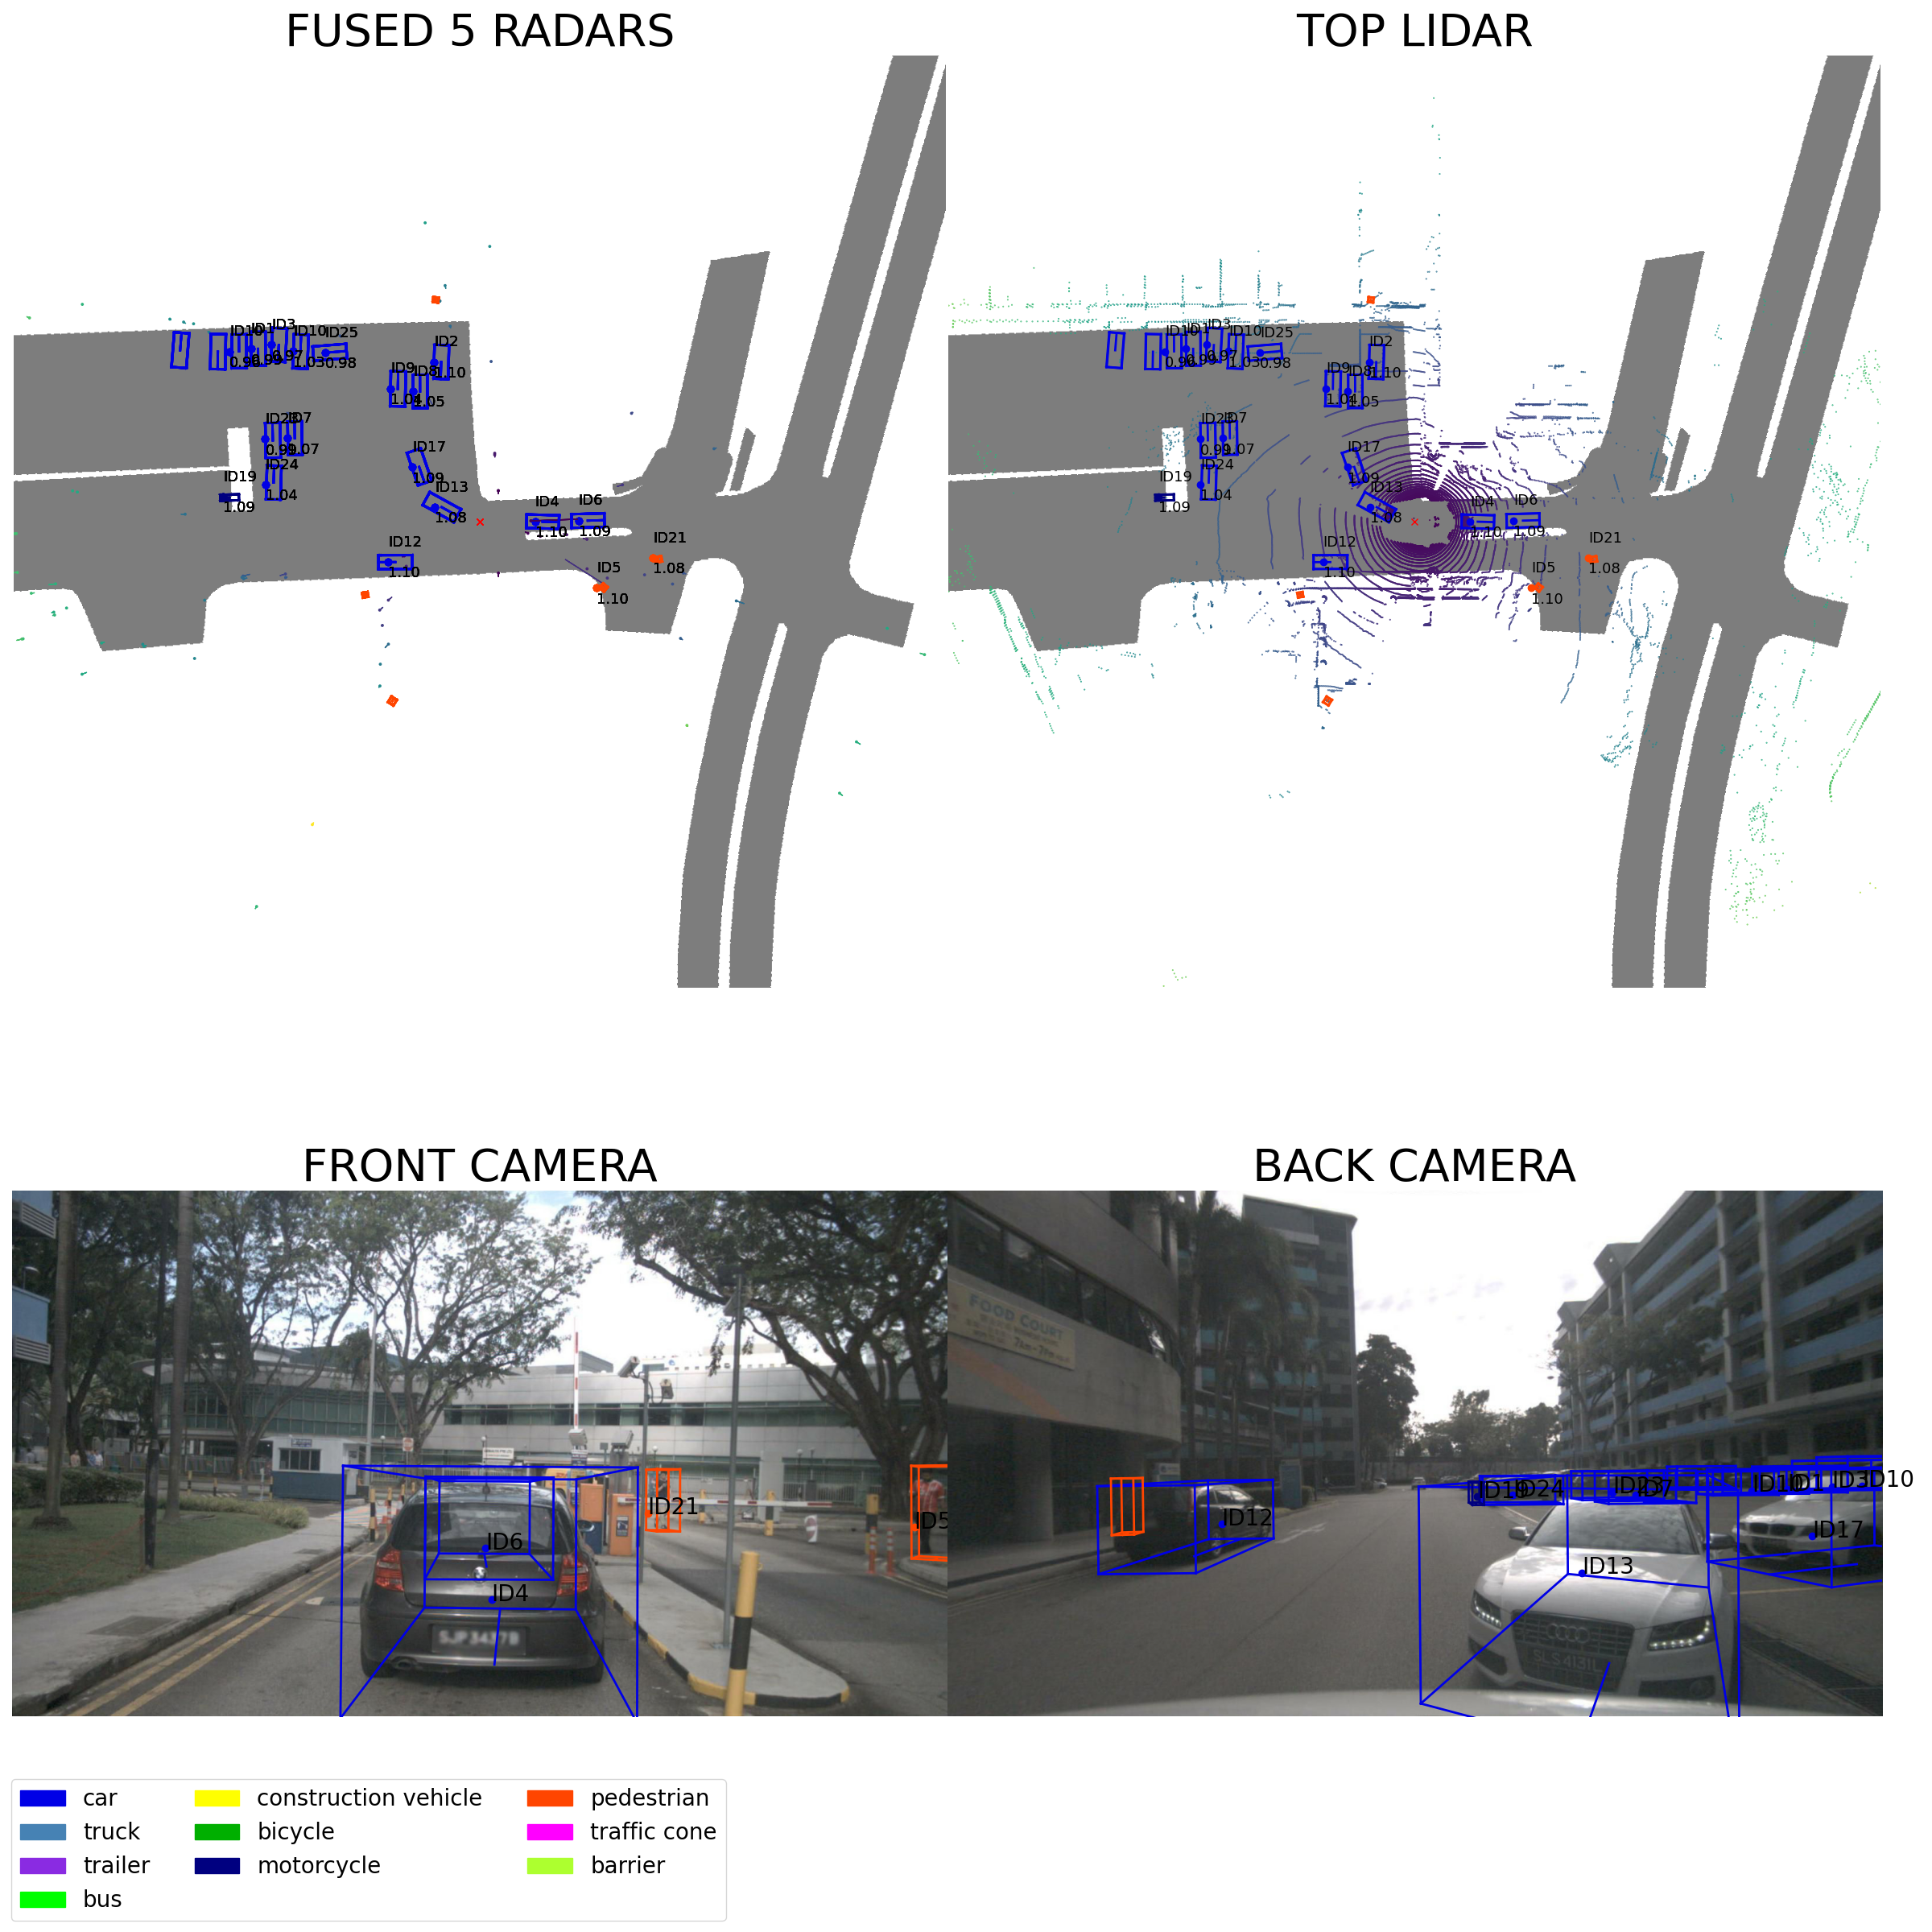
\includegraphics[width=0.5\linewidth]{GNN/3.png}
    \end{figure}
\end{frame}

\begin{frame}{Primary Metrics One: AMOTA}
\begin{itemize}
\item{larger is better}
\item{AMOTA, metrics for entire scene, n frames}
\item{$AMOTA=\frac{1}{n-1} \sum_r MOTAR$}
\item{MOTAR, metrics for single frame}
\item{$MOTAR=max(0,1-\frac{IDS_r+FP_r+FN_r-(1-r)P}{r*P})$}
\item{$r=\frac{i}{n-1}$ i = (1,2,...n-1)}
\end{itemize}
\end{frame}
\begin{frame}{Primary Metrics One: AMOTA}
\begin{itemize}
\item{IDS, ID switch. Any IDS would cause MORTA to decrease}
\item{FP, False Positive. Any FP would cause MORTA to decrease}
\item{FN, False Negative. Any FN would cause MORTA to decrease}
\item{P, number of ground-truth. Normalizing element}
\end{itemize}
\end{frame}
\begin{frame}{Primary Metrics Two: AMOTP}
\begin{itemize}
\item{Smaller is better}
\item{$\frac{1}{n-1}\sum_r \frac{\sum_{it} d_{it}}{\sum_{t} TP_{t}}$}
\item{$r=\frac{i}{n-1}$ i = (1,2,...n-1)}
\item{$d_{it}$, position error for track i at time t. Any position error would lead to increase of AMOTP}
\item{$TP_{t}$ Track Matched at time t. Normalizing Element}
\end{itemize}. 
\end{frame}
\begin{frame}{Result}
    \begin{table}
        \begin{tabular}{l l l l}
            \toprule
            Metrics & Regular & $P_d$ replaced & Label\\
            \midrule
            \textcolor{red}{AMOTA}        &0.020 & 0.019          &0.031               \\
            \textcolor{red}{AMOTP}     &1.879   & 1.900          & 1.846               \\
            RECALL     &0.132    & 0.096           & 0.173               \\
            MOTAR     &0.103    & 0.134          & 0.306               \\
            GT     &17080    & 17080          & 17080               \\
            MOTA     &0.025    & 0.027          & 0.043               \\
            MOTP     &0.815    & 1.056          & 0.604               \\
            MT     &334    & 264           & 372               \\
            ML     &5951    & 6598           & 5525               \\
            
            FAF     &194.4    & 231.9          & 108.7              \\
            TP     &22130    & 16360          & 17184               \\
            FP     &16341    & 4435          & 11992               \\

            \bottomrule
        \end{tabular}
    \end{table}
\end{frame}


\begin{frame}{Result}
    \begin{table}
        \begin{tabular}{l l l l}
            \toprule
            Metrics & Regular & $P_d$ replaced & Label\\
            \midrule
            FN     &94172    & 101114         & 88575               \\
            IDs     &3263    & 2091          & 13803               \\
            FRAG     &1785    & 968           & 3320               \\
            TID     &7.77    & 10.2           & 5.57               \\
            LGD     &9.12    & 11.22           & 6.7             \\

            \bottomrule
        \end{tabular}
    \end{table}
\end{frame}


\end{document}